\graphicspath{{./assets/}}
\setcounter{mtc}{4}
\chapter{2nd Sprint: Information gathering and cloud design }
\fancyhead[R]{\ungaramond\small\textbf{Chapter IV. 2nd Sprint: Information gathering and cloud design }}
\minitoc
\newpage

\section*{Introduction}

\section{Sprint backlog :}

\begin{longtable}[H]{|m{1.5cm}|m{3cm}|m{1.5cm}|m{8cm}|}
\hline
{\textbf{Epic ID}} & {\textbf{Epic}} & {\textbf{Story ID}} & {\textbf{Story}}\\
\hline
1  & Information gathering.	 &  1.1	 &  Research provider specific (OVH) constraints\\
\cline{3-4}
& & 1.2 & Container orchestration choice. \\
\cline{3-4}
& & 1.3	& Deciding on virtualized networking. \\
\cline{3-4}
& & 1.4	& Deciding on application load balancer. \\
\cline{3-4}
& & 1.5	& Deciding on network level load balancer. \\
\cline{3-4}
& & 1.6	& Storage backend choice.\\
\hline
\caption{2nd sprint backlog}
\end{longtable}


\section{Package diagram of cloud resources :}

The cluster resources are basically cloud instances with different specifications tailored to their use cases. Three major groups of resources are distinguished in the following diagram: Control plane instances, Compute instances and storage assets which are object store buckets and compute instances to which raw block stores are attached. 

\begin{figure}[H]\centering
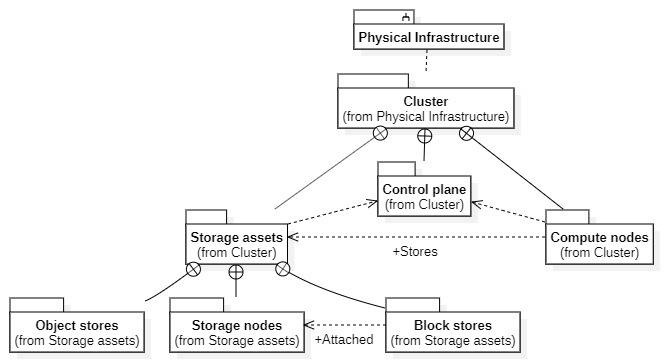
\includegraphics[width=1.0\textwidth,angle=00]{assets/f11.jpg}
\caption{Package diagram of cloud resources }
\label{fig:Package diagram of cloud resources }
\end{figure}

\section{Comparative study on container orchestrators: }

Container Orchestration Engines such as “Kubernetes”, “Apache Mesos” and “docker swarm” are platforms for managing containers and automating the deployment, scaling, and operations of containers across a cluster of nodes. This is achieved by pooling the discrete cloud resources into a single PaaS on which workloads can be deployed. 

\begin{longtable}[H]{|m{3.5cm}|m{3.5cm}|m{3.5cm}|m{3.5cm}|}
\hline
Criteria & Kubernetes & Docker swarm & Apache Mesos  \\
\hline
Ease of use & Medium & Easy & Complex  \\
\hline
Cluster scalability & Medium to Large & Small to Medium & Very Large  \\
\hline
Cluster installation & Complex & Easy & Medium  \\
\hline
Container deployment & YAML based  & Docker based & JSON based \\
\hline
Community Support  & Large  & Moderate  & Small \\
\hline
Configuration & Declarative  & Declarative & Imperative \\
\hline
\caption{Sprint planification}
\end{longtable}

Kubernetes is our container orchestration tool of choice in this project. It is known for its highly advanced orchestration capabilities, built-in load balancing, rolling updates, and self-healing. It has a declarative configuration model and a highly extensible architecture. However, it does have a steeper learning curve compared to Docker Swarm.  

Our goal is to tackle the task of establishing a fully sustainable PaaS by utilizing its flexibility via custom resource definitions. 


\section{Package diagram for the PaaS logical components:}

\begin{figure}[H]\centering
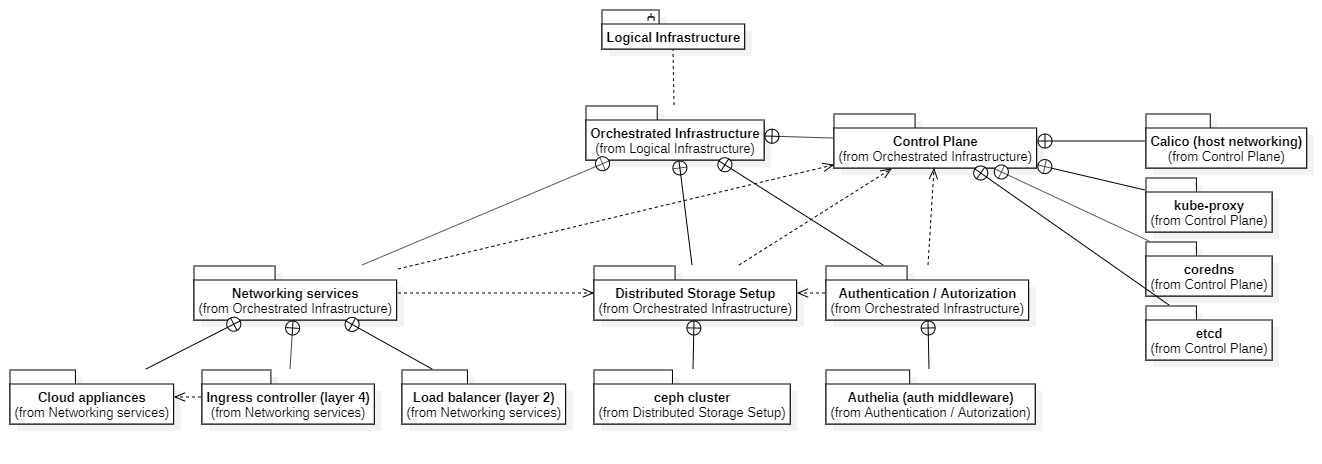
\includegraphics[width=1.0\textwidth,angle=00]{assets/f12.jpg}
\caption{Package diagram for the PaaS logical components}
\label{fig:Package diagram for the PaaS logical components}
\end{figure}

This figure illustrates a package design of the main PaaS services. We mainly distinguish: 
\begin{itemize}[label={--}]
\item  A control plane: which manages assets in the cluster, namely, nodes, pods and other api resources. 
\item An assortment of networking services which allow for ingress control in both the network and application layers. 
\item An authentication and authorization service: which is aimed to control access to the cluster. 
\item A distributed, scalable, and replicated storage backend which is independent of the infrastructure in place to provide data redundancy and disaster recovery. 
\end{itemize}

\section*{Conclusion}
In conclusion, designing a PaaS environment in the cloud requires careful planning and information gathering to ensure that the resulting architecture is scalable, secure, and cost-effective. 

The design process should start with identifying the business requirements and user needs, as well as understanding the technical requirements of the application workloads. This information can then be used to identify the necessary cloud services and tools needed to build and deploy the PaaS environment. 

Once the cloud services and tools are identified, the design process can proceed to developing the cloud architecture. This architecture should take into account scalability, resiliency, and security, and should be designed to support the specific application workloads. It's important to properly architect the network topology, select appropriate storage solutions, and design for automated deployment and management.